\section{Supervised Learning}\label{sec:supervised-learning}

Supervised Learning is the task of turning a dataset of input-output
pairs into a general rule that should be able to produce the correct
output even for inputs not necessarily seen in the original dataset.

The inputs and outputs are usually denoted respectively with the
symbols \(x\) and \(y\).
Therefore, our rule will be the function \(f\) for which we would
like \(y = f(x)\).

\subsection{Dataset}
A dataset is a collection of unordered \textit{observations} of
input/output pairs.
Each input is composed of a set of \textit{features} or
\textit{attributes}, while the outputs contain \textit{labels}
or \textit{targets}.
Generally the inputs contain many features while the outputs are
scalar values and every input and output of the dataset has the same
features and labels,
however this needn't hold true.

Suppose that the examples of the dataset have \(n\) features and that
the number of examples in the dataset is \(m\). The dataset can be
represented as a pair of matrices \(X\) and \(Y\) where \(X\) is \(m
\times n\) and \(Y\) is \(m \times 1\). The convention is to
represent vectors as columns, so the rows of \(X\) will be the
transposed input vectors.

The features and the label can be categorized into:
\begin{itemize}
  \item \textbf{Categorical}: For example relationship status
    (married, single, divorced, \dots)
  \item \textbf{Real-valued}: For example weight or height
  \item \textbf{Binary}: Boolean values (true/false, 0/1, yes/no, \dots)
\end{itemize}

As already stated, the goal is to produce a rule that generalizes
well to the examples so that it can work on yet-unseen ones. This rule is called a
\textit{classifier} if the label is categorical, whereas it is called
a \textit{regressor} if it is real-valued.

\subsection{Assumptions of supervised learning} \label{sec:assumptions-supervised-learning}
We assume that the input/output examples contained in the dataset are
chosen at random from
the target population (the dataset is technically a \textit{sample}
of the population).
Another assumption we make is that examples of the dataset are
independent from each other and belong to the same
distribution, which is called \textbf{IID Assumption} (independent
and identically distributed).
This assumption is quite strong and will also be discuted later in
\ref{sec:vanilla-fl}

\subsection{Common Approach to Supervised Learning}
A common approach to supervised learning is the so-called
\textit{discriminative approach}, which involves the following steps:
\begin{enumerate}
  \item Define an error measurement.
  \item Define a hypothesis space, which is the set of all the rules
    that we can accept.
  \item Pick the rule inside the hypothesis space for which the error
    on the training set is minimized.
\end{enumerate}

This approach has its own pitfalls: we might choose a rule that
matches perfectly the training set but does not generalize well. This
is called \textit{overfitting} and can be seen in \ref{fig:overfitting}
polynomial below. The opposite of this is called
\textit{underfitting}.
\begin{figure}[h!]
  \centering
  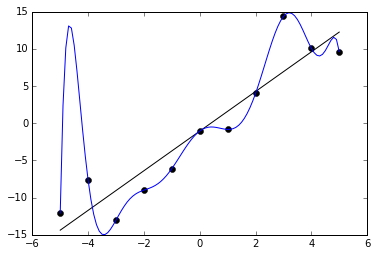
\includegraphics[width=0.8\textwidth]{figures/ml/overfitted_data.png}
  \caption[Overfitted data visualization]{Overfitted data visualization. One can see that the
    polynomial fits perfectly the training set but does likely not
  generalize well.}
  \begin{minipage}{0.8\textwidth}
    \begin{center}
      \footnotesize
      Source:
      \href{https://commons.wikimedia.org/wiki/File:Overfitted_Data.png}{Wikimedia
      Commons}, licensed under CC BY-SA 4.0.
    \end{center}

  \end{minipage}
  \label{fig:overfitting}
\end{figure}
To mitigate this problem, we split the data into the \textbf{training
set} and the \textbf{testing set}. The former is used for training
our model and creating our rule, whereas the latter is used solely
for testing our rule.
